\newif\ifglobal

%%%%%%%%%%%%%%%%%%%%%%%
%%% Compile to view %%%
%%%%%%%%%%%%%%%%%%%%%%%

%%%%%%%%%%%%%%%%%%%%%%%%%%%%%%%%%%%%%%%%%%%%%%%%%%%
%%% Readme:                                     %%%
%%% https://www.overleaf.com/read/bwdjvfjksvjy/ %%%
%%%%%%%%%%%%%%%%%%%%%%%%%%%%%%%%%%%%%%%%%%%%%%%%%%%

% >>> M?: marks a module setting number or important notice

% >>> M4: Set {./relative-path} to external files for this module <<<
\def \modulefiles {./38-WCTRL}
% To add an external file, use:
% (Replace '---' with actual filename)
% '\input{\modulefiles/tables/---.tex}' for tables
% '\includegraphics{\modulefiles/figures/---}' for figures
% '\subfile{\modulefiles/---}' for register files

% >>> M1: This module is in global project? <<<
% 'YES' - uncomment; 'NO' - comment out
\globaltrue

\ifglobal
    \documentclass[main\_\_EN.tex]{subfiles}

\else    \documentclass[openany, 10pt]{book}

    % >>> M2: In ./00-shared/preamble-trm-module, also find
    %         settings for visibility of todo notes, watermark <<<
    \usepackage{preamble-trm-module}

    % >>> M3: Temporary labels in English,
    %         you can add your own labels there <<<
    \myexternaldocument{./00-shared/temp-labels-en}


\fi %\ifglobal


\setcounter{secnumdepth}{4}

% >>> M5: If this module needs any updates in
% './00-shared/preamble-trm-module.sty'
% (include additional package, etc.), contact your module PM
% or create the file './00-shared/changelog.tex' make the
% necessary updates yourself and document them in this file <<<

\begin{document}


% Sets language into which pre-defined bits of text are translated
\selectlanguage{english}

% Do not delete this block
\ifglobal
% Add the following front matter if
% this module is outside of global project
\else
    \InputIfFileExists{readme}{}{}
    {\let\clearpage\relax \listoftodos}
    \tableofcontents
    %\listoftables
    %\listoffigures
\fi

%%%%%%%%%%%%%%%%%%%%%%%%%
%%% TRM Module Begins %%%
%%%%%%%%%%%%%%%%%%%%%%%%%

\hypertarget{wctrl}{}
\chapter{World Controller (WCL)}\label{mod:wctrl}
\section{Introduction}
\chipname{} allows users to allocate its hardware and software resource into Secure World (World0) and Non-secure World (World1), thus protecting resource from unauthorized access (read or write), and from malicious attacks such as malware, hardware-based monitoring, hardware-level intervention, and so on. CPUs can switch between Secure World and Non-secure World with the help of the World Controller.

By default, all resource in \chipname{} are shareable. Users can allocate the resource into two worlds by managing respective permission (For details, please refer to Chapter \ref{mod:permctrl} \textit{\nameref{mod:permctrl}}). This chapter only introduces the World Controller and how CPUs can switch between worlds with the help of World Controller.

\section{Features}
\label{sec:alias-features}

\chipname{}'s World Controller:
\begin{itemize}
    \item Controls the CPUs to switch between the Secure World and Non-secure World
    \item Logs CPU's world switches
    \item Allows NMI masking
    \item Allows independent world switches of CPUs (CORE\_\regindex{m}: CPU0 and CPU1)
\end{itemize}

\section{Functional Description}
\label{sec:38-WCTRL-func-descr}

With the help of World Controller, we can allocate different resources to the Secure World and the Non-secure World:

\begin{itemize}
    \item Secure World (World0):
    \begin{itemize}
        \item Can access all peripherals and memories;
        \item Performs all confidential operations, such as fingerprint identification, password processing, data encryption and decryption, security authentication, etc.
    \end{itemize}
    \item Non-secure World (World1):
    \begin{itemize}
        \item Can access some peripherals and memories;
        \item Performs other operations, such as user operation and different applications, etc.
    \end{itemize}
\end{itemize}


\chipname{}'s CPU and slave devices are both configurable with permission to either Secure World and/or Non-Secure World:
\begin{itemize}
    \item CPU can be in either world at a particular time:
        \begin{itemize}
            \item In Secure World: performs confidential operations;
            \item In Non-secure World: performs non-confidential operations;
            \item By default, CPU runs in Secure World after power-up, then can be programmed to switch between two worlds.
        \end{itemize}
    \item All slave devices (including peripherals\hyperref[note:wctrl-access]{*} and memories) can be configured to be accessible from the Secure World and/or the Non-secure World:
        \begin{itemize}
            \item Secure World Access: this slave can be called from Secure World only, meaning it can be accessed only when CPU is in Secure World;
            \item Non-secure World Access: this slave can be called from Non-secure World only, meaning it can be accessed only when CPU is in Non-secure World.
            \item Note that a slave can be configured to be accessible from both Secure World and Non-secure World simultaneously.
        \end{itemize}
    For details, please refer to Chapter \ref{mod:permctrl} \textit{\nameref{mod:permctrl}}.
\end{itemize}

\begin{tiplisting}
\label{note:wctrl-access}
* World Controller itself is a peripheral, meaning it also can be granted with Secure World access and/or Non-secure World access, just like all other peripherals. However, to secure the world switch mechanism, World Controller should not be accessible from Non-secure world. Therefore, world controller \textbf{should not be granted with} Non-secure World access, preventing any modification to world controller from the Non-secure World.
\end{tiplisting}

\textbf{When CPU accesses any slaves:}

\begin{enumerate}
    \item First, CPU notifies the salve about its own world information;
    \item Second, slave decides if it can be accessed by CPU based on the CPU's world information and it's own world permission configuration.
        \begin{itemize}
        \item if allowed, then this slave responds to CPU;
        \item if not allowed, then this slave will not respond to CPU and trigger an interrupt.
        \end{itemize}
\end{enumerate}
In this way, the resources in the Secure World will not be illegally accessible by the Non-secure World in an unauthorized way.

\clearpage
\section{CPU's World Switch} \label{sec:38-WCTRL-recommended-operation}

CPU can switch from Secure World to Non-secure World, and from Non-secure World to Secure World.

\subsection{From Secure World to Non-secure World}\label{sec:38-WCTRL-safe-nosafe-switch}

\begin{figure}[H]
    \centering
    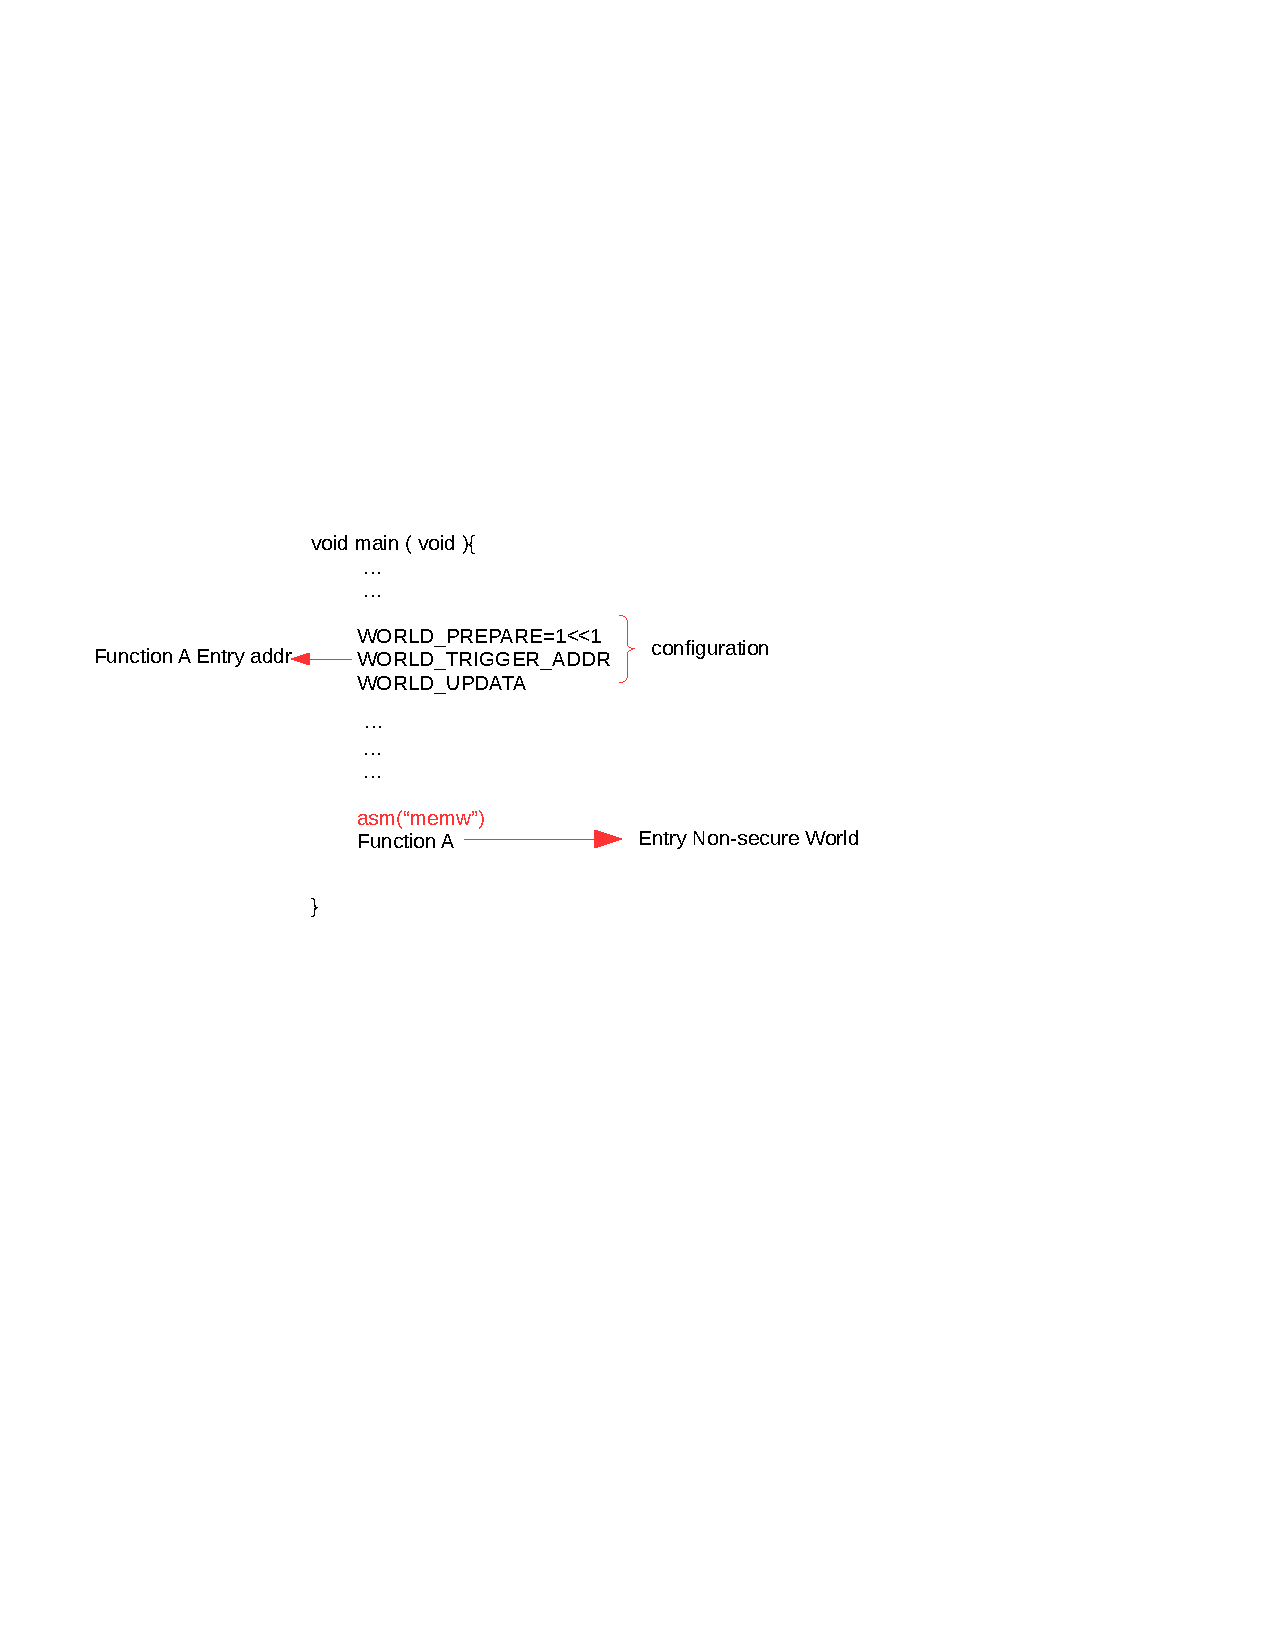
\includegraphics[width=0.7\textwidth]{./38-WCTRL/figures/world0toworld1.pdf}
    \caption{Switching From Secure World to Non-secure World}
    \label{fig:38-WCTRL-safe-nosafe-switch}
\end{figure}
\chipname{}'s CPU only needs to complete the following steps to switch from Secure World to Non-secure World:
\begin{enumerate}
    \item Configure the World Controller, as described below.
    \item Clear the data stored in write\_buffer, as described in Section \ref{sec:wctrl-writer-buffer}.
\end{enumerate}

After that, CPU can switch to the Non-secure World.

However, it's worth noting that you cannot call the application in Non-secure world immediately after configuring the World Controller. For reasons such as CPU pre-indexed addressing and pipeline, it is possible that the CPU have already executed the application in Non-secure World before the World Controller configuration is effective, meaning the CPU runs unsecured application in the Secure World.

Therefore, you need to make sure the CPU only calls applications in the Non-secure world after the World Controller configuration takes effect. This can be guaranteed by \textbf{declaring the applications in the Non-secure World as ``noinline"}.


\subparagraph{Configuring the World Controller}

The steps to configure the World Controller to switch the CPU from the Secure World to the Non-secure World are described below:
\begin{enumerate}
    \item Write 0x{}2 to Register \hyperref[regdesc:WCLCORE0WORLDPREPAREREG]{WCL\_CORE\_\regindex{m}\_WORLD\_PERPARE\_REG}, indicating the CPU needs to switch to the Non-secure World.
    \item Configure Register \hyperref[regdesc:WCLCORE0WORLDTRIGGERADDRREG]{WCL\_CORE\_\regindex{m}\_World\_TRIGGER\_ADDR\_REG} as the entry address to the Non-secure World, i.e., the address of the application in the Non-secure World that needs to be executed.
    \item Write any value to Register \hyperref[regdesc:WCLCORE0WORLDUPDATEREG]{WCL\_CORE\_\regindex{m}\_World\_UPDATE\_REG}, indicating the configuration is done.
\end{enumerate}

\begin{tiplisting}\label{note:38-WCTRL-safe2unsafe}
\vspace{-2em}
\begin{itemize}
    \item Register \hyperref[regdesc:WCLCORE0WORLDUPDATEREG]{WCL\_CORE\_\regindex{m}\_World\_UPDATE\_REG}  must be configured at last.
    \item Registers \hyperref[regdesc:WCLCORE0WORLDPREPAREREG]{WCL\_CORE\regindex{m}\_WORLD\_PERPARE\_REG} and \hyperref[regdesc:WCLCORE0WORLDTRIGGERADDRREG]{WCL\_CORE\_\regindex{m}\_World\_TRIGGER\_ADDR\_REG} can be configured in any order.
    \item After the configuration, you also need to use assembly instruction memw (memory wait) to clear write\_buffer. For details, see Section \ref{sec:wctrl-writer-buffer}.
\end{itemize}
\end{tiplisting}

Afterwards, the World Controller keeps monitoring if CPU is executing the configured address of the application in Non-secure World. CPU switches to the Non-secure World once it executes the configured address, and executes the applications in the Non-secure World.

After configuration, the World Controller:
\begin{itemize}
    \item Keeps monitoring until the CPU executes the configured address and switches to the Non-secure World.
    \begin{itemize}
        \item Write any value to Register \hyperref[regdesc:WCLCORE0WORLDCANCELREG]{WCL\_CORE\_\regindex{m}\_World\_Cancel\_REG} to cancel the World Controller configuration. After the cancellation, CPU will not switch to the Non-secure World even it executes to the configured address. Note that you also need to use assembly instruction memw (memory wait) to clear write\_buffer. For details, see Section \ref{sec:wctrl-writer-buffer}.
    \end{itemize}
    \item The World Controller can only switch from the Secure World to Non-secure World once per configuration. Therefore, the World Controller needs to be configured again after each world switch to prepare it for the next world switch.
\end{itemize}

\subsection{From Non-secure World to Secure World}\label{sec:38-WCTRL-nosafe-safe-switch}

\begin{figure}[H]
    \centering
    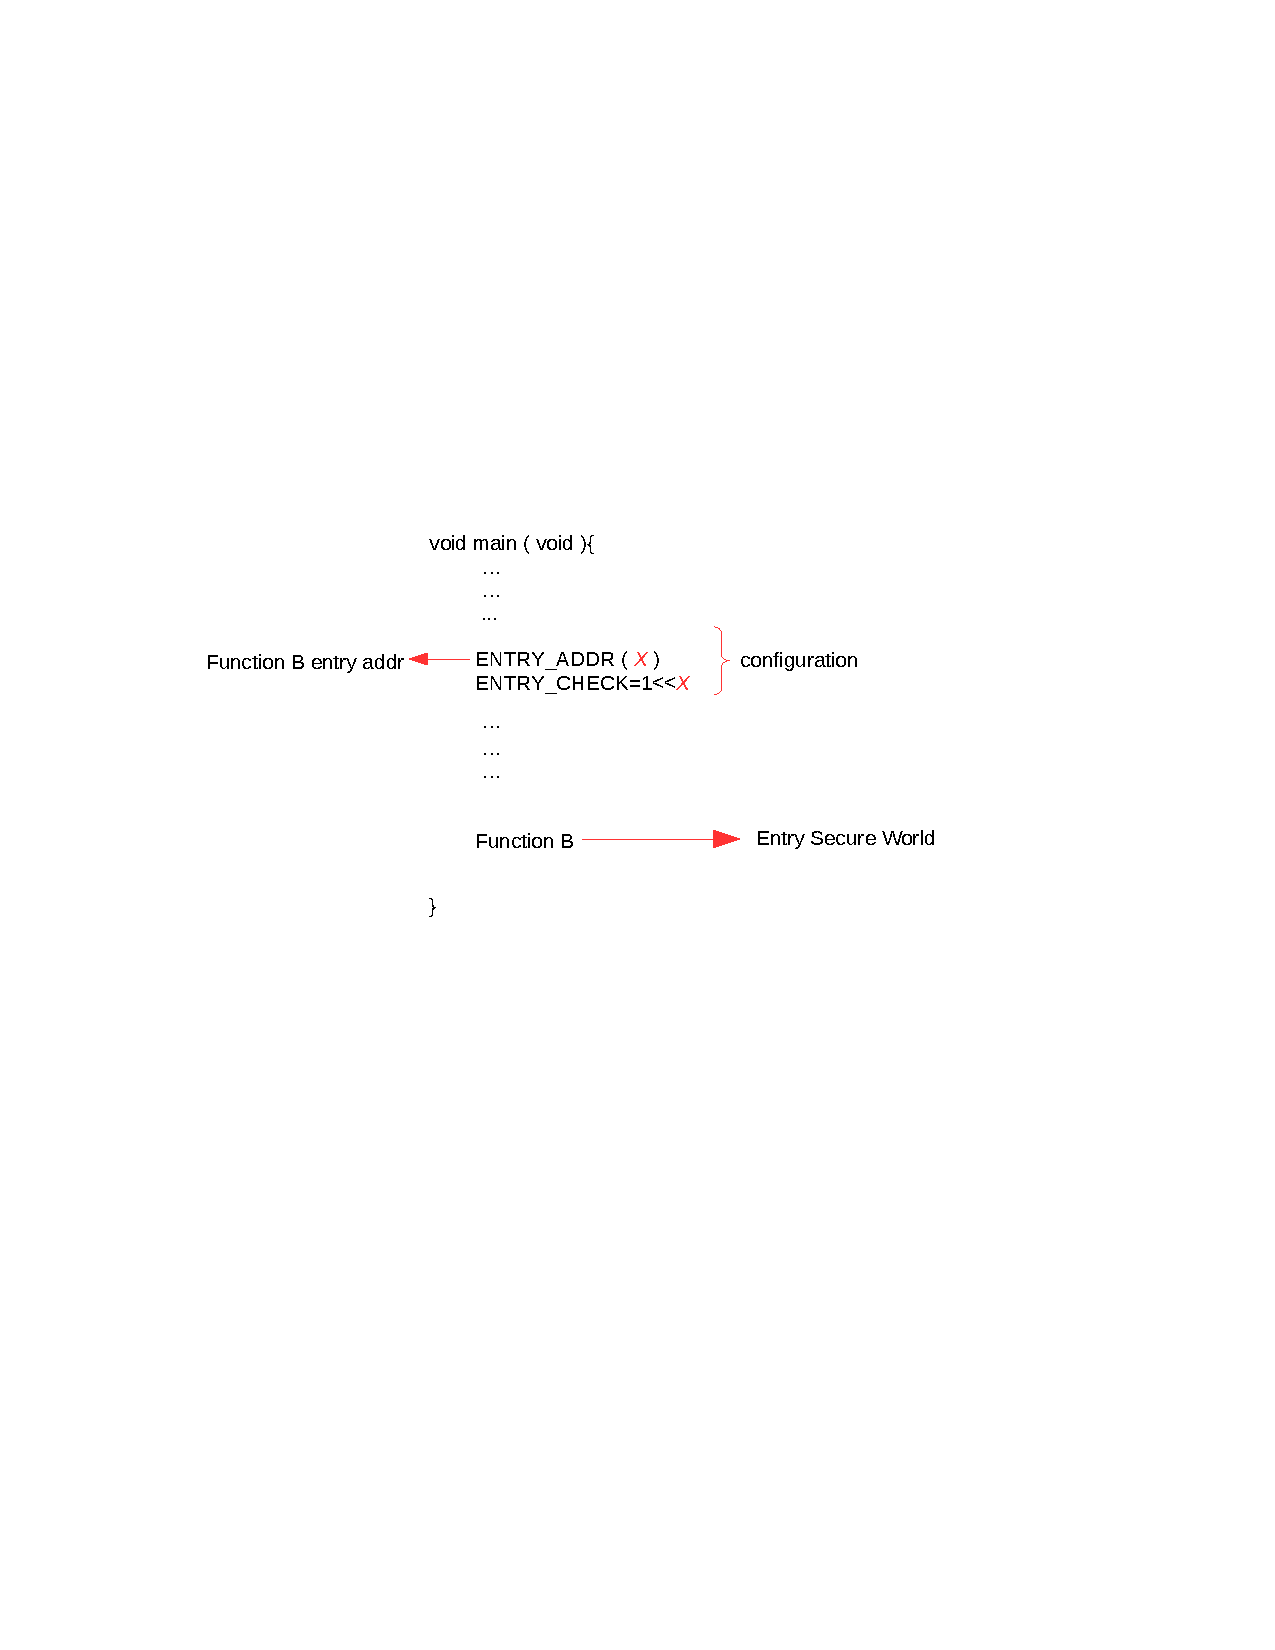
\includegraphics[width=0.8\textwidth]{./38-WCTRL/figures/world1toworld0.pdf}
    \caption{Switching From Non-secure World to Secure World}
    \label{fig:38-WCTRL-nosafe-safe-switch}
\end{figure}

CPU can only switch from Non-secure World to Secure World via \textbf{Interrupts (or Exceptions)}. After configuring the World Controller, the CPU can switch back Non-secure World to Secure World upon the configured Interrupt trigger.

See details below:

\begin{enumerate}
    \item Configure Registers \hyperref[regdesc:WCLCORE0MESSAGEADDRREG]{WCL\_CORE\_\regindex{m}\_MESSAGE\_ADDR\_REG} and \hyperref[regdesc:WCLCORE0MESSAGEMAXREG]{WCL\_CORE\_\regindex{m}\_MESSAGE\_MAX\_REG} to clear write\_buffer, as described in Section \ref{sec:wctrl-writer-buffer}.
    \item Configure Registers \hyperref[regdesc:WCLCORE0ENTRYnADDRREG]{WCL\_CORE\_\regindex{m}\_ENTRY\_\regindex{n}\_ADDR\_REG (\regindex{n}: 1-13)} as the entry address of interrupts (or exceptions).
    \begin{itemize}
        \item Note that all of \chipname{}'s interrupts and exceptions are using VecBase + offset as its address. Therefore, you need to configure \hyperref[regdesc:WCLCORE0ENTRYnADDRREG]{WCL\_CORE\_\regindex{m}\_ENTRY\_\regindex{n}\_ADDR\_REG (\regindex{n}: 1-13)} whenever you modify the VecBase.
    \end{itemize}
    \item Configure Register \hyperref[regdesc:WCLCORE0ENTRYCHECKREG]{WCL\_CORE\_\regindex{m}\_ENTRY\_CHECK\_REG} to enable the monitor of a certain entry. In this way, the CPU switches to the Secure World immediately when it executes the address monitored at this particular entry.
    \begin{itemize}
        \item Bit \regindex{x} controls the entry monitoring of Entry \regindex{x} (\hyperref[regdesc:WCLCORE0ENTRYnADDRREG]{WCL\_CORE\_\regindex{m}\_ENTRY\_\regindex{x}\_ADDR\_REG}). You can enable monitoring for more than one entry.
        \begin{itemize}
            \item 0: Disable monitoring
            \item 1: Enable monitoring
        \end{itemize}
        \item Register \hyperref[regdesc:WCLCORE0ENTRYCHECKREG]{WCL\_CORE\_\regindex{m}\_ENTRY\_CHECK\_REG} is effective after configuration all the time till it's disabled, meaning you don't need to configure this register every time after each world switch.
    \end{itemize}
\end{enumerate}
\subsection{Clearing the write\_buffer}\label{sec:wctrl-writer-buffer}

\chipname{} has implemented \href{https://en.wikipedia.org/wiki/Write_buffer}{write\_buffer}, which means the CPU buses can still hold some data from or execute instructions from the other world after world switches. To improve data security, we need to clear the writer\_buffer before world switching:
\begin{itemize}
    \item \textbf{Switching from Secure World to Non-secure World}
    \begin{itemize}
        \item Use assembly instruction memw (memory wait).
    \end{itemize}
    \item \textbf{Switching from Non-secure World to Secure World}
    \begin{itemize}
        \item Switch CPU data bus:
        \begin{enumerate}
        \item Pre-configure the following registers:
        \begin{itemize}
            \item Configures Register \hyperref[regdesc:WCLCORE0MESSAGEADDRREG]{WCL\_CORE\_\regindex{m}\_MESSAGE\_ADDR\_REG} to an address in the Non-secure World;
        \item Configure Register \hyperref[regdesc:WCLCORE0MESSAGEMAXREG]{WCL\_CORE\_\regindex{m}\_MESSAGE\_MAX\_REG} to \regindex{Z} (\begin{math} Z \in \{ 3, 4, \dots, 16 \end{math}\})
        \end{itemize}
        \item Write sequences of 0, 1, \dots, \regindex{Z-1}, \regindex{Z} to the address configured in Register \\ \hyperref[regdesc:WCLCORE0MESSAGEADDRREG]{WCL\_CORE\_\regindex{m}\_MESSAGE\_ADDR\_REG} before world switching. For example, if \regindex{Z} is configured to 3, then you need to write sequences of 0, 1, 2, 3 into the configured address; if \regindex{Z} is 5, then write  0, 1, 2, 3, 4, 5.
        \item Afterwards, the CPU will switch its data bus to the other world once it detects the agreed sequences configured in \hyperref[regdesc:WCLCORE0MESSAGEMAXREG]{WCL\_CORE\_\regindex{m}\_MESSAGE\_MAX\_REG} are being written to the agreed address configured in \hyperref[regdesc:WCLCORE0MESSAGEADDRREG]{WCL\_CORE\_\regindex{m}\_MESSAGE\_ADDR\_REG}.
    \end{enumerate}
    \end{itemize}
\end{itemize}


\section{World Switch Log} \label{subsub:world_switch_table}

In actual use cases, CPU is switching between two worlds quite frequently and has to deal with nested interrupts. To be able to restore to the previous world, World Controller keeps a world switching log in a series of registers, which is called ``World Switch Log Table".


\subsection{Structure of World Switch Log Register}

\chipname{}'s World Switch Log Table consists of 13 \hyperref[regdesc:WCLCORE0STATUSTABLEnREG]{WCL\_CORE\_\regindex{m}\_STATUSTABLE\regindex{n}\_REG(\regindex{n}: 1-13)} registers (see Figure \ref{fig:wcl-world-status}). The world switching of address configured in \hyperref[regdesc:WCLCORE0ENTRYnADDRREG]{WCL\_CORE\_\regindex{m}\_ENTRY\_\regindex{x}\_ADDR\_REG}, which is monitored at Entry \regindex{x}, is logged in \hyperref[regdesc:WCLCORE0STATUSTABLEnREG]{WCL\_CORE\_\regindex{m}\_STATUSTABLE\regindex{x}\_REG}.

\begin{figure}[H]
    \centering
    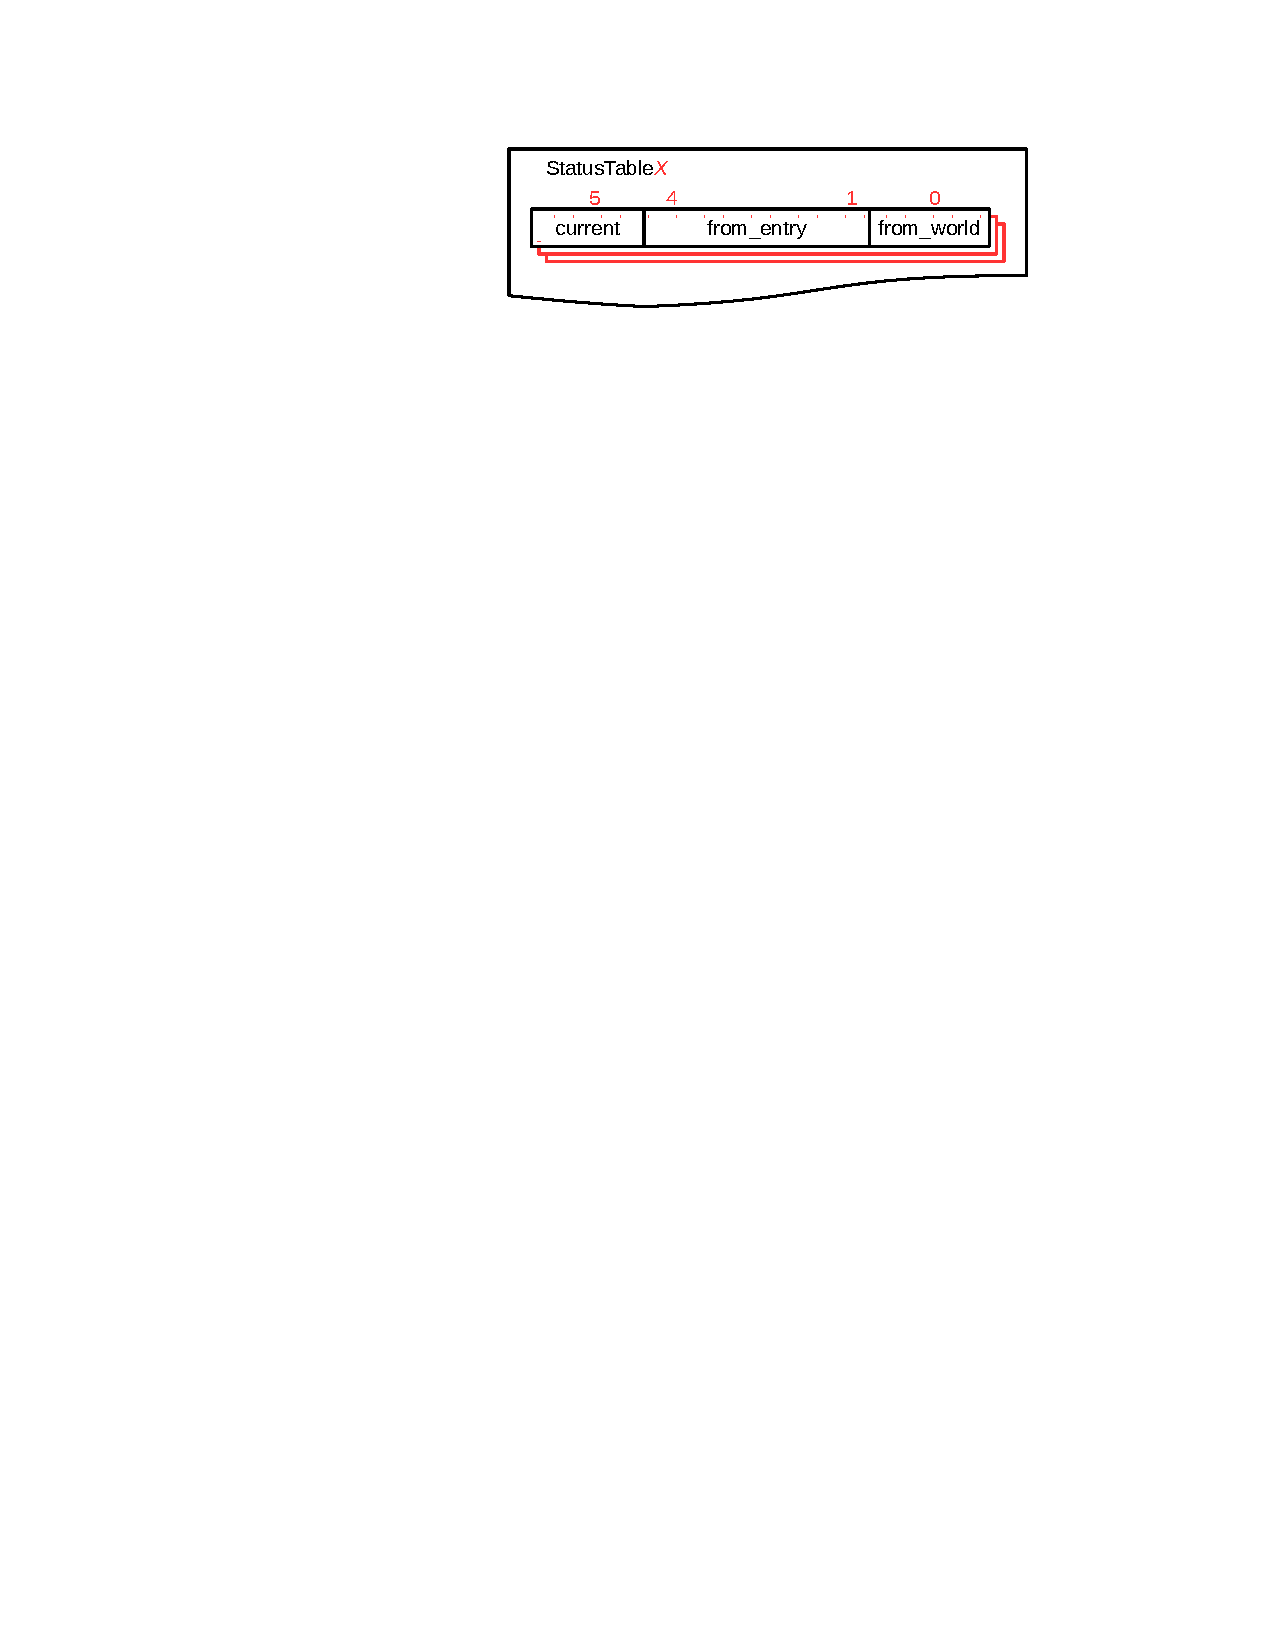
\includegraphics[width=0.5\textwidth]{./38-WCTRL/figures/statustable.pdf}
    \caption{World Switch Log Register}
    \label{fig:wcl-world-status}
\end{figure}

\begin{itemize}
    \item \hyperref[fielddesc:WCLCORE0FROMWORLDn]{WCL\_CORE\_\regindex{m}\_FROM\_WORLD\_\regindex{n}}: logs the world information before the world switch.
    \begin{itemize}
        \item 0: CUP was in Secure World
        \item 1: CPU was in Non-secure World
    \end{itemize}
    \item \hyperref[fielddesc:WCLCORE0FROMENTRYn]{WCL\_CORE\_\regindex{m}\_FROM\_ENTRY\_\regindex{n}}: logs the entry information before the world switch.
    \begin{itemize}
        \item 0: CPU was not at any interrupts monitored at any entry.
        \item 1 - 13: CPU was at the interrupt monitored at a certain entry.
    \end{itemize}
    \item \hyperref[fielddesc:WCLCORE0CURRENTn]{WCL\_CORE\_\regindex{m}\_CURRENT\_\regindex{n}}: indicates if CPU is at the interrupt monitored at the current entry. When CPU is at the interrupt monitored at Entry \regindex{x}, \begin{itemize}
        \item  \hyperref[fielddesc:WCLCORE0CURRENTn]{WCL\_CORE\_\regindex{m}\_CURRENT\_\regindex{x}} is updated to 1,
        \item and the same fields of all other entries are updated to 0.
    \end{itemize}
\end{itemize}

\subsection{How World Switch Log Registers Are Updated}\label{sec:wctrl-update-statetable}

To explain this process, assuming:
\begin{enumerate}
    \item At the beginning:
    \begin{itemize}
        \item CPU is running in the Non-secure World;
        \item Registers \hyperref[regdesc:WCLCORE0STATUSTABLEnREG]{WCL\_CORE\_\regindex{m}\_STATUSTABLE\regindex{n}\_REG(\regindex{n}: 1-13)} are all empty.
    \end{itemize}
    \item Then an interrupt occurs at Entry 9;
    \item Then another interrupt with higher priority occurs at Entry 1;
    \item Then the last interrupt with highest priority occurs at Entry 4.
\end{enumerate}

The World Switch Log Table is updated as described below:
\begin{enumerate}
    \item First, an interrupt occurs at Entry 9. At this time, CPU executes to the entry address of this interrupt. The World Switch Log Table is updated as described in Figure \ref{fig:wcl-world-change0}:
    \begin{figure}[H]
    \centering
    
\includegraphics[width=0.3\textwidth]{./38-WCTRL/figures/world_table0.eps}
    \caption{Nested Interrupts Handling - Entry 9}
    \label{fig:wcl-world-change0}
    \end{figure}
    \begin{itemize}
        \item \hyperref[regdesc:WCLCORE0STATUSTABLEnREG]{WCL\_CORE\_\regindex{m}\_STATUSTABLE9\_REG}
        \begin{itemize}
            \item Field \hyperref[fielddesc:WCLCORE0FROMWORLDn]{WCL\_CORE\_\regindex{m}\_FROM\_WORLD\_9} is updated to 1, indicating CPU was in Non-secure World before the interrupt.
            \item Field \hyperref[fielddesc:WCLCORE0FROMENTRYn]{WCL\_CORE\_\regindex{m}\_FROM\_ENTRY\_9} is updated to 0, indicating there was not any interrupt before this one.
            \item Field \hyperref[fielddesc:WCLCORE0CURRENTn]{WCL\_CORE\_\regindex{m}\_CURRENT\_9} is updated to 1, indicating the CPU is currently at the interrupt monitored at Entry 9.
        \end{itemize}
        \item Other \hyperref[regdesc:WCLCORE0STATUSTABLEnREG]{WCL\_CORE\_\regindex{m}\_STATUSTABLE\regindex{n}\_REG} registers are not updated.    \end{itemize}
    \item Then another interrupt with higher priority occurs at Entry 1. At this time, CPU executes to the entry address of this interrupt. The World Switch Log Table is updated again as described in Figure \ref{fig:wcl-world-change1}:     \begin{figure}[H]
        \centering
        
\includegraphics[width=0.3\textwidth]{./38-WCTRL/figures/world_table1.eps}
        \caption{Nested Interrupts Handling - Entry 1}
        \label{fig:wcl-world-change1}
        \end{figure}
    \begin{itemize}
        \item \hyperref[regdesc:WCLCORE0STATUSTABLEnREG]{WCL\_CORE\_\regindex{m}\_STATUSTABLE1\_REG}
        \begin{itemize}
            \item Field \hyperref[fielddesc:WCLCORE0FROMWORLDn]{WCL\_CORE\_\regindex{m}\_FROM\_WORLD\_1} is updated to 0, indicating the CPU was in Secure World before this interrupt.
            \item Field \hyperref[fielddesc:WCLCORE0FROMENTRYn]{WCL\_CORE\_\regindex{m}\_FROM\_ENTRY\_1} is updated to 9, indicating the CPU was executing the interrupt at Entry 9.
            \item Field \hyperref[fielddesc:WCLCORE0CURRENTn]{WCL\_CORE\_\regindex{m}\_CURRENT\_1} is updated to 1, indicating CPU is currently at the interrupt monitored at Entry 1.
        \end{itemize}
        \item \hyperref[regdesc:WCLCORE0STATUSTABLEnREG]{WCL\_CORE\_\regindex{m}\_STATUSTABLE9\_REG}
        \begin{itemize}
            \item Field \hyperref[fielddesc:WCLCORE0CURRENTn]{WCL\_CORE\_\regindex{m}\_CURRENT\_9} is updated to 0, indicating CPU is no longer at the interrupt monitored at Entry 9 (Instead, CPU is at the interrupt monitored at Entry 1 already).
            \item Fields \hyperref[fielddesc:WCLCORE0FROMWORLDn]{WCL\_CORE\_\regindex{m}\_FROM\_WORLD\_9} and \hyperref[fielddesc:WCLCORE0FROMENTRYn]{WCL\_CORE\_\regindex{m}\_FROM\_ENTRY\_9} stay the same.
        \end{itemize}
        \item Other \hyperref[regdesc:WCLCORE0STATUSTABLEnREG]{WCL\_CORE\_\regindex{m}\_STATUSTABLE\regindex{n}\_REG} registers are not updated.
    \end{itemize}
        \item Then the last interrupt with highest priority occurs at Entry 4. At this time, CPU executes to the entry address of interrupt 4. The World Switch Log Table is updated again as described in Figure \ref{fig:wcl-world-change2}:
        \begin{figure}[H]
            \centering
            
\includegraphics[width=0.3\textwidth]{./38-WCTRL/figures/world_table2.eps}
            \caption{Nested Interrupts Handling - Entry 4}
            \label{fig:wcl-world-change2}
        \end{figure}

        \begin{itemize}
        \item \hyperref[regdesc:WCLCORE0STATUSTABLEnREG]{WCL\_CORE\_\regindex{m}\_STATUSTABLE4\_REG}
        \begin{itemize}
            \item Field \hyperref[fielddesc:WCLCORE0FROMWORLDn]{WCL\_CORE\_\regindex{m}\_FROM\_WORLD\_4} is updated to 0, indicating the CPU was in Secure World before this interrupt.
            \item Field \hyperref[fielddesc:WCLCORE0FROMENTRYn]{WCL\_CORE\_\regindex{m}\_FROM\_ENTRY\_4} is updated to 1, indicating the CPU was the interrupt at Entry 1.
            \item Field \hyperref[fielddesc:WCLCORE0CURRENTn]{WCL\_CORE\_\regindex{m}\_CURRENT\_4} is updated to 1, indicating the CPU is currently at the interrupt monitored an Entry 4.
        \end{itemize}
        \item \hyperref[regdesc:WCLCORE0STATUSTABLEnREG]{WCL\_CORE\_\regindex{m}\_STATUSTABLE1\_REG}
        \begin{itemize}
            \item Field \hyperref[fielddesc:WCLCORE0CURRENTn]{WCL\_CORE\_\regindex{m}\_CURRENT\_1} is updated to 0, indicating the CPU is no longer at the interrupt monitored at Entry 1 (Instead CPU is at the interrupt monitored at Entry 4 already).
            \item Fields \hyperref[fielddesc:WCLCORE0FROMWORLDn]{WCL\_CORE\_\regindex{m}\_FROM\_WORLD\_1} and \hyperref[fielddesc:WCLCORE0FROMENTRYn]{WCL\_CORE\_\regindex{m}\_FROM\_ENTRY\_1} are not updated.
        \end{itemize}
        \item Other \hyperref[regdesc:WCLCORE0STATUSTABLEnREG]{WCL\_CORE\_\regindex{m}\_STATUSTABLE\regindex{n}\_REG} registers are not updated.
\end{itemize}
\end{enumerate}

\subsection{How to Read World Switch Log Registers} \label{sec:wctrl-read-table}

By reading World Switch Log Registers, we get to understand the information of previous world switches and nested interrupts, thus being able to restore to previous world.

Steps are described below: (See Figure \ref{fig:wcl-world-change2} as an example):
\begin{enumerate}
    \item Read Register \hyperref[regdesc:WCLCORE0STATUSTABLECURRENTREG]{WCL\_CORE\_\regindex{m}\_STATUSTABLE\_CURRENT\_REG}, and understand CPU is now at the interrupt monitored at Entry 4.
    \item  Read 1 from Field \hyperref[fielddesc:WCLCORE0FROMENTRYn]{WCL\_CORE\_\regindex{m}\_FROM\_ENTRY\_4}, and understand the CPU was at an interrupt monitored at Entry 1.
    \item Read 9 from Field \hyperref[fielddesc:WCLCORE0FROMENTRYn]{WCL\_CORE\_\regindex{m}\_FROM\_ENTRY\_1}, and understand the CPU was at an interrupt monitored at Entry 9.
    \item Read 0 from \hyperref[fielddesc:WCLCORE0FROMENTRYn]{WCL\_CORE\_\regindex{m}\_FROM\_ENTRY\_9}, and understand CPU wasn't at any interrupt. Then read 1 from \hyperref[fielddesc:WCLCORE0FROMWORLDn]{WCL\_CORE\_\regindex{m}\_FROM\_WORLD\_9}, and understand CPU was in Non-secure World at the beginning.
\end{enumerate}


\subsection{Nested Interrupts}

\chipname{} supports nested interrupts, for example:

\begin{enumerate}
    \item An interrupt A occurs. CPU jumps to interrupt A entry, which triggers world switches.
    \item When CPU is handling interrupt A, an  interrupt B with higher priority occurs.
    \item Then the CPU drops the current interrupt A and switches to the higher priority interrupt B first.
    \item After returning from interrupt B, CPU resumes executing the instruction at interrupt A entry, which triggers world switches again.
\end{enumerate}

In this way, CPU executes the entry address of the first interrupt twice (one time when the interrupt occurs and another time when CPU returns to this interrupt), and thus triggering the world switches twice, which inevitably leads to multiple records tracked for the same interrupt in \nameref{subsub:world_switch_table} and prevents the CPU from restoring to the previous world correctly.


\subsubsection{How to Handle Nested Interrupts}

To avoid multiple records being logged incorrectly in the \nameref{subsub:world_switch_table}, the following actions must be completed:

\begin{itemize}
    \item During the design stage, add two assembly instruction NOP.N (No Operation) to the vector entrance of all interrupts and exceptions.
    \item During the execution, update the address where the interrupts return to following the instructions described in \ref{sec:wctrl-prog-step}.
\end{itemize}

In this way, when returning to the interrupt at Entry \regindex{B}, the interrupt monitored at Entry \regindex{A} will not return to the entry address of Entry \regindex{B}, but the address after the NOP instructions, thus preventing to trigger the world controller unexpectedly. Also, the NOP instruction doesn't do anything, so nothing is changed even when the NOP instructions are skipped.

\subsubsection{Programming Procedure}\label{sec:wctrl-prog-step}

\textbf{Handling the interrupt at Entry \regindex{A}: \label{step:wctrl-start-interrput}}
    \begin{enumerate}
        \item Clear the write\_buffer by writing the agreed sequences configured in Register \hyperref[regdesc:WCLCORE0MESSAGEMAXREG]{WCL\_CORE\_\regindex{m}\_MESSAGE\_MAX\_REG} to the address configured in  \hyperref[regdesc:WCLCORE0MESSAGEADDRREG]{WCL\_CORE\_\regindex{m}\_MESSAGE\_ADDR\_REG}. For details, see Section \ref{sec:wctrl-writer-buffer}.
        \item Execute the interrupt programs. \label{step:interrupt-process-normal}
        \item Disable all interrupts.
        \item Update the address where the interrupt at Entry \regindex{A} returns to: \label{step:interrupt_process_update}
        \begin{itemize}
            \item Read Field \hyperref[fielddesc:WCLCORE0FROMENTRYn]{WCL\_CORE\_\regindex{m}\_FROM\_ENTRY\_\regindex{A}} for Entry \regindex{A}:
            \begin{itemize}
                \item 0: indicates all interrupts are handled, and returns to a normal program:
                \begin{enumerate}
                    \item Update Field \hyperref[fielddesc:WCLCORE0CURRENTn]{WCL\_CORE\_\regindex{m}\_CURRENT\_\regindex{A}} of Entry \regindex{A} to 0, indicating the CPU is no longer at the interrupt monitored at Entry \regindex{A}.
                    \item Go to Step \ref{step:last-step}.
                \end{enumerate}
                \item 1 - 13: indicates the CPU returns to another interrupt monitored at Entry \regindex{B},
                \begin{enumerate}
                    \item First, check the return address of the interrupt at Entry \regindex{A}:
                    \begin{itemize}
                        \item If it points to the first NOP.N instruction of the interrupt at Entry \regindex{B}, then add 4 to the return address of the interrupt at Entry \regindex{A}.
                        \item If it points to the second NOP.N instruction of the interrupt at Entry \regindex{B}, then add 2 to the return address of the interrupt at Entry \regindex{A}.
                        \item If it points to other address, then no need to update the return address.
                    \end{itemize}
                    \item Update the \nameref{sec:wctrl-read-table}:
                    \begin{itemize}
                        \item Update the world switch register of Entry \regindex{A}:
                        \begin{itemize}
                            \item Update Field \hyperref[fielddesc:WCLCORE0CURRENTn]{WCL\_CORE\_\regindex{m}\_CURRENT\_\regindex{A}} to 0, indicating the CPU is no longer at the interrupt monitored at Entry \regindex{A}.
                            \item Fields \hyperref[fielddesc:WCLCORE0FROMWORLDn]{WCL\_CORE\_\regindex{m}\_FROM\_WORLD\_\regindex{A}} and \hyperref[fielddesc:WCLCORE0FROMENTRYn]{WCL\_CORE\_\regindex{m}\_FROM\_ENTRY\_\regindex{A}} stay the same.
                        \end{itemize}
                        \item Update the  world switch register of Entry \regindex{B}:
                        \begin{itemize}
                            \item Update Field  \hyperref[fielddesc:WCLCORE0CURRENTn]{WCL\_CORE\_\regindex{m}\_CURRENT\_\regindex{B}} to 1, indicating the CPU will return to Entry \regindex{B}.
                        \end{itemize}
                     \end{itemize}
            \end{enumerate}
            \end{itemize}
        \end{itemize}
        \item Prepare to exit interrupt.\label{step:last-step}
            \begin{enumerate}
                \item Check if CPU needs to switch to the other world:
                    \begin{itemize}
                        \item If world switch not required, then go to Step \ref{step:final}.
                        \item If world switch required, then switch the CPU to the other world following instructions described in Section \ref{sec:38-WCTRL-recommended-operation}, then go to Step \ref{step:final}.
                    \end{itemize}
            \end{enumerate}
        \item Enable interrupts, and exit. \label{step:final}
\end{enumerate}


\begin{tiplisting}
Steps \ref{step:interrupt_process_update} and \ref{step:last-step} should not be interrupted by any interrupts. Therefore, users need to disable all the interrupts before these steps, and enable interrupts once done.
\end{tiplisting}

\section{NMI Interrupt Masking}

Some software process of \chipname{} should not be interrupted. For example, the configuration of World Controller should not be interrupted by any interrupts, including the NMI interrupts.

Normally, we can configure some CPU registers to mask different kinds of interrupts, but NMI interrupt is not one of them. To mask an NMI interrupt, you need to configure the interrupt sources, which is more complicated. For details, see Chapter \ref{mod:intmtrx} \textit{\nameref{mod:intmtrx}}.

World Controller has implemented some hardware mechanism to simplify the process to mask NMI interrupts for:
\begin{itemize}
    \item \textbf{All} applications:
    \begin{itemize}
        \item Configure \hyperref[fielddesc:WCLCORE0NMIMASK]{WCL\_CORE\_\regindex{m}\_NMI\_MASK}:
            \begin{itemize}
            \item 1: Enable
            \item 0: Disable
            \end{itemize}
    \end{itemize}
    \item \textbf{Some} applications:
        \begin{enumerate}
            \item Configures \hyperref[fielddesc:WCLCORE0NMIMASKTRIGGERADDR]{WCL\_CORE\_\regindex{m}\_NMI\_MASK\_TRIGGER\_ADDR} to the address at which the NMI interrupt masking ends, meaning the CPU stops masking NMI interrupts after this address.
            \item Write any value to \hyperref[fielddesc:WCLCORE0NMIMASKDISABLE]{WCL\_CORE\_\regindex{m}\_NMI\_MASK\_DISABLE}, indicating the completion of TRIGGER\_ADDR configuration.            \item Write any value to  \hyperref[fielddesc:WCLCORE0NMIMASKENABLE]{WCL\_CORE\_\regindex{m}\_NMI\_MASK\_ENABLE} to start masking NMI interrupts till the address configured in \hyperref[fielddesc:WCLCORE0NMIMASKTRIGGERADDR]{WCL\_CORE\_\regindex{m}\_NMI\_MASK\_TRIGGER\_ADDR}.
        \end{enumerate}
\end{itemize}

\begin{tiplisting}
\vspace{-2em}
 \begin{itemize}
    \item Only one of the above two methods should be used at the same time.
    \item The configuration to mask NMI interrupts is effective all the time until trigger address executes. Therefore, you need to configure the world controller to mask NMI interrupts again once trigger address executes.
 \end{itemize}
\end{tiplisting}

\clearpage

\section{Register Summary}\hypertarget{wctrl-reg-summ}{}
The addresses in this section are relative to the World Controller base address provided in Table \ref{tab:sysmem-base-address} in Chapter \ref{mod:sysmem} \textit{\nameref{mod:sysmem}}.

Note that, the table below only lists the registers for CPU0. CPU1 shares exactly the same set of registers. Adding 0x{}0400 to the offset of the equivalent of CPU0 register gives you address for CPU1 registers.

For example, the offset for CPU0 register \hyperref[regdesc:WCLCORE0ENTRYCHECKREG]{WCL\_CORE\_0\_ENTRY\_CHECK\_REG} is 0x{}007C, the offset for CPU1 equivalent \hyperref[regdesc:WCLCORE0ENTRYCHECKREG]{WCL\_CORE\_1\_ENTRY\_CHECK\_REG} should be 0x{}007C + 0x{}0400, which is 0x{}047C.

The abbreviations given in Column \textbf{Access} are explained in Section \hyperref[glossary-access-types]{\textit{Access Types for Registers}}.

\subfile{\modulefiles/38-WCTRL-reg-summ__EN}


\clearpage

\section{Registers}

The addresses in this section are relative to the World Controller base address provided in Table \ref{tab:sysmem-base-address} in Chapter \ref{mod:sysmem} \textit{\nameref{mod:sysmem}}.

Note that, the section below only lists the registers for CPU0. CPU1 shares exactly the same set of registers. Adding 0x{}0400 to the offset of the equivalent of CPU0 register gives you address for CPU1 registers.

For example, the offset for CPU0 register \hyperref[regdesc:WCLCORE0ENTRYCHECKREG]{WCL\_CORE\_0\_ENTRY\_CHECK\_REG} is 0x{}007C, the offset for CPU1 equivalent \hyperref[regdesc:WCLCORE0ENTRYCHECKREG]{WCL\_CORE\_1\_ENTRY\_CHECK\_REG} should be 0x{}007C + 0x{}0400, which is 0x{}047C.

\subfile{\modulefiles/38-WCTRL-reg__EN}

\end{document}
